\textbf{مورد استفاده:}
حذف رزومه
\\
\textbf{شرح مختصر :UC}
در این قسمت فریلنسر رزومه خود حذف می‌کند.
\\
\textbf{پيش شرط:}
ورود به مدیریت رزومه در داشبورد فریلنسر.
\\
\textbf{سناريو اصلی:}
\begin{enumerate}
	\item
	شروع
	\item
	فریلنسر دکمه حذف رزومه را انتخاب می‌کند و سیستم اطلاعات را به فریلنسر نمایش می‌دهد.
	\item
		فریلنسر تایید حذف رزومه را به سیستم ارسال می‌کند.
	\item
		سیستم رزومه را بررسی و از بانک اطلاعات حذف می‌کند.
	\item
	پایان
\end{enumerate}

\noindent
\textbf{پس شرط:}
ندارد.
\\
\textbf{سناريوهای فرعی:}
\\
\textbf{سناريو فرعی 1:}
رزومه با موفقیت حذف شود
\\
\textbf{شرح مختصر :UC}
این سناریو در مرحله ۴ سناریو اصلی در صورت موفقیت آمیز بودن حذف رزومه اجرا می‌شود.
\begin{enumerate}
	\item
	شروع
	\item
	اطلاعات فرم بررسی می‌شود و یک پیغام به فریلنسر نمایش داده می‌شود که اطلاعات با موفقیت حذف شده است.
	\item
	از مرحله 4 سناریو اصلی ادامه پیدا می‌کند.
	\item
	پایان
\end{enumerate}

\noindent
\textbf{پس شرط:}
ندارد.



\begin{figure}[H]
	\centering
	\includegraphics[width=0.7\textwidth]{Diagram/2.Activity/فریلنسر/مدیریت-رزومه-حذف.png}
	\caption{دیاگرام فعالیت حذف رزومه}
	\label{fig:a:حذف-رزومه}
\end{figure}
\begin{figure}[H]
	\centering
	\includegraphics[width=0.7\textwidth]{Diagram/3.StateMachine/فریلنسر/مدیریت-رزومه-حذف.png}
	\caption{دیاگرام حالت ماشین حذف رزومه}
	\label{fig:sm:حذف-رزومه}
\end{figure}
\begin{figure}[H]
	\centering
	\includegraphics[width=1\textwidth]{Diagram/4.Collaboration/1.Sequence/فریلنسر/مدیریت-رزومه-حذف.png}
	\caption{دیاگرام توالی حذف رزومه}
	\label{fig:s:حذف-رزومه}
\end{figure}
\begin{figure}[H]
	\centering
	\includegraphics[width=0.9\textwidth]{Diagram/4.Collaboration/2.Communication/فریلنسر/مدیریت-رزومه-حذف.png}
	\caption{دیاگرام همکار حذف رزومه}
	\label{fig:c:حذف-رزومه}
\end{figure}
